\section{Methods}
\frame{\tableofcontents[currentsection, hideothersubsections]}

\begin{frame}
\frametitle{Methods}
DDPG (=DPG+DQN)~\cite{Lillicrap2015} components:
\begin{itemize}
  \item Deterministic Policy-Gradient (DPG) \cite{Silver2014}
  \item Deep Q-Network (DQN= QLearning + deepLearning) \cite{Mnih2013}
  \item Actor-Critic Methods \cite{Sutton1998}
\end{itemize}

\end{frame}

\begin{frame}
\frametitle{Methods: DPG \cite{Silver2014}}

DPG: Deterministic Policy Gradient, an actor-critic approach:
\begin{itemize}
  \item actor: $\mu (s|\theta^{\mu})$,
  specifies the current policy by deterministically mapping states to a specific action
  \item critic: $Q(s, a)$,
  learned using the Bellman equation as in Q-learning.
\end{itemize}

Update $\theta^{\mu}$ by applying the chain rule to the expected return from
the start distribution, $J$, with respect to the actor parameters, $\theta^{\mu}$:
\begin{equation} \label{equ:policy_grad}
\begin{split}
\nabla_{\theta^{\mu}} J &  \approx \mathbb{E}_{s_t \sim \rho^{\beta}} \Big[ \nabla_{\theta^{\mu}} Q(s,a|\theta^Q) |_{s = s_t, a = \mu(s_t|\theta^{\mu})} \Big] \\
  & = \mathbb{E}_{s_t \sim \rho^{\beta}} \Big[ \nabla_{\theta^{\mu}} Q(s,a|\theta^Q) |_{s = s_t, a = \mu(s_t)} \nabla_{\theta^{\mu}} \mu(s|\theta^{\mu})|_{s = s_t} \Big]
\end{split}
\end{equation}

Equ.~\ref{equ:policy_grad} is the policy gradient (the gradient of the policy's performance),
in practice the discount in $\rho^{\beta}$ is ignored.
\end{frame}

\begin{frame}
\frametitle{Methods: Replay-buffer, as in DQN~\cite{Mnih2013}}
Why:
\begin{itemize}
\item NN assumes iid samples;\\
the samples from exploring sequentially in an environment are not iid
\item to make efficient use of hardware optimizations:\\
to learn in minibatches rather than (fully) online
\end{itemize}
\vspace{5mm}

What:
\begin{itemize}
  \item replay buffer contains $(s_t, a_t, r_t, s_{t+1})$ sampled from $E$ using an exploration policy
  \item At each timestep the actor and critic are updated by sampling a minibatch uniformly from the buffer
% Because DDPG is an off-policy algorithm, the replay buffer can be large, allowing the algorithm to benefit from learning across a set of uncorrelated transitions.
\end{itemize}

\end{frame}

\begin{frame}
\frametitle{Method: Fix target network}
Why:
\begin{itemize}
\item Q-learning (eq.\ref{equ:qloss}) with NN is unstable, \\
since the network $Q(s, a|\theta^Q)$ being updated is also used in
calculating the target value, $y$
\end{itemize}

What:
\begin{itemize}
\item create a copy of the actor and critic networks, i.e. \\
  $Q'(s, a|\theta^{Q'})$ and $µ'(s|\theta^{\mu'})$
\item use those for calculating the target values
\item target networks update: \\
    $\theta' \leftarrow \tau \theta + (1 - \tau) \theta'$ with $\tau \ll 1$\\
    (warn: may slow learning, since the target network delays the propagation of value estimations, but
    in practice, this was greatly outweighed by the stability of learning)
\end{itemize}

\end{frame}


\begin{frame}
\frametitle{Method: Feature scaling: batch normalization}
Why:
\begin{itemize}
\item different components of the observation may have different physical units (for example, positions versus velocities)
\item their ranges may vary across environments
% \item make it difficult
%   a) for the network to learn effectively
%   b) to find hyper-parameters which generalise across environments with different scales of state values.
% \item to minimize covariance shift during training, by ensuring that each layer receives whitened input
\end{itemize}
\vspace{3mm}

What:
\begin{itemize}
\item normalizes each dimension across the samples in a minibatch to have unit mean and variance.
\item maintains a running average of the mean and variance to use for normalization during testing
(during xploration or evaluation)
\end{itemize}

\end{frame}

\begin{frame}
\frametitle{Method: Exploration}
Why:\\
Exploration-exploitation dillema
\vspace{5mm}

What:\\
Construct an exploration policy $\mu^x$ by adding noise sampled from
a noise process $\mathcal{N}$ to our actor policy:
$\mu^{xplor} = \mu(s_t | \theta^{\mu}_t) + \mathcal{N}$.

\end{frame}

\begin{frame}
\frametitle{Method: Deep DPG Algo}
\begin{figure}
    \centering
    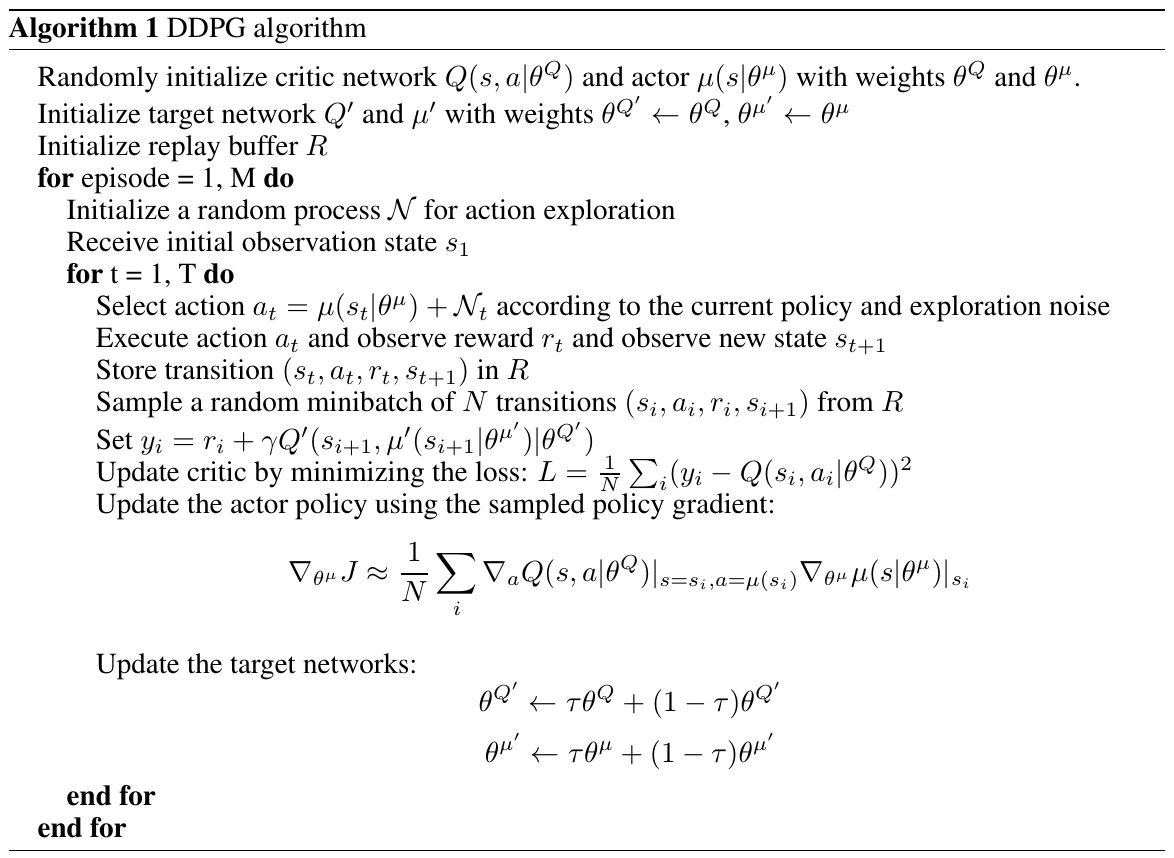
\includegraphics[scale=0.35]{ddpg_algo}
\end{figure}
\end{frame}
